\documentclass[10pt,a4paper]{article}
\usepackage[utf8]{inputenc}
\usepackage[T1]{fontenc}
\usepackage{amsmath,amssymb,amsfonts}
\usepackage{graphicx}
\usepackage{hyperref}
\usepackage{algorithm}
\usepackage{algpseudocode}
\usepackage{multicol}
\usepackage{geometry}
\usepackage{cite}
\usepackage{authblk}
\usepackage{mathtools, empheq}
\usepackage{booktabs}
\usepackage{lipsum}
\geometry{margin=2cm}

\title{Beyond Income: Simulating the End of Work}
\author{Fabien Furfaro}
\date{\today}

% ------------------------------------------------------------------------
% Style Reminder Helper (For AI Assistant): Keep every sentence in abstracts and main text neutral, humble, and scientific.

% Write in ENGLISH only

% For each sentence, check for "marketing" tone (e.g., overuse of words like "novel", "substantial", "robust") or subjective point of view (e.g., "traditionnal", "essential")
% and replace with more cautious, evidence-based claims.
%
% Prefer:
% - "show", "suggest", "may improve", "offers potential", "addresses some limitations"
% - "To the best of our knowledge...", "Preliminary experiments suggest...", 
%   "Further investigation is needed...", "This approach may be of interest..."
%

% Apply rules : Less is More 

% Avoid:
% - "groundbreaking", "revolutionary", "unprecedented", "definitively demonstrates",
%   overly strong claims without empirical or theoretical backing
%
% Make explicit:
% - Limitations, resource constraints, preliminary or ongoing nature of results,
%   encouragement for community replication and extension.

% Example sentences:
% - "We propose a novel architecture..." → "We propose an alternative architecture..."
% - "Substantially improves..." → "Shows promising results..." / "May improve..."
% - "Our approach is fully robust..." → "Preliminary results suggest some robustness..."
%
% Always use conditional language ("could", "might", "suggests") when appropriate and prefer cautious claims.
% Before finalizing, review each sentence with these criteria in mind.
% ------------------------------------------------------------------------


\begin{document}

\maketitle

\begin{abstract}
The rapid emergence of Artificial General Intelligence (AGI) and advanced automation may profoundly reshape economic structures, labor markets, and wealth distribution worldwide. This paper provides an analysis of the macroeconomic and social consequences of AGI-driven automation within a unified modeling framework combining extended Cobb--Douglas production functions and game-theoretic firm-level simulations. Preliminary results suggest that while AGI unlocks significant productivity gains, it simultaneously erodes the labor income base sustaining consumer demand, potentially creating a paradox of abundance with collapsing consumption. We evaluate Universal Basic Income (UBI) as possible redistributive mechanisms. Our findings indicate that, absent proactive intervention, AGI could induce systemic inequality and economic instability. This study also conceptualizes  Merit-Based Income (MBI) as a transitional tool and a cultural institution that may foster social recognition and prepare society for a post-economic paradigm. Further investigation is needed to address economic, social, and ecological challenges for a just and stable transition toward a future where value transcends market exchange.
\end{abstract}

\tableofcontents

\section{Introduction}
Artificial General Intelligence (AGI) is characterized by its ability to perform human-level cognitive and physical tasks across diverse domains. This technological development differs from prior automation waves, which mostly replaced routine or manual labor but left cognitive, creative, and interpersonal work largely intact. AGI may render large portions of human labor economically obsolete, triggering complex socio-economic transformations. This raises a critical question: AGI could generate unprecedented productivity, but by displacing labor, it may also erode the primary source of consumer income, potentially threatening market stability.

This study addresses this issue through a combined theoretical and empirical approach. We build on recent research \cite{OpenAI2023,StanfordAI2025,MIT2025} and propose a refined macroeconomic and microeconomic framework to analyze automation dynamics, employment outcomes, and redistribution strategies in AGI-impacted economies. Our contributions include:

\begin{itemize}
    \item Development of a game-theoretic model capturing firm-level automation incentives under competitive pressure, revealing a Prisoner's Dilemma dynamic that may lead to over-automation.
    \item Integration of this micro-level model into an extended Cobb--Douglas macroeconomic framework accounting for labor displacement and resulting demand fluctuations.
    \item Simulation-based evaluation of two redistribution mechanisms: Universal Basic Income (UBI) and Merit-Based Income (MBI), assessing their potential to stabilize demand and foster social cohesion.
    \item Exploration of MBI’s role as a cultural institution supporting societal transition toward a post-economic era.
\end{itemize}

The remainder of this paper is structured as follows. Section 2 reviews relevant literature; Section 3 describes the theoretical models and simulation methodology; Section 4 presents results; Section 5 discusses implications and policy; Section 6 concludes.

\section{Literature Review}
The labor market impact of AI technologies, including language models and robotics, has been extensively studied. OpenAI (2023) estimates that 80\% of U.S. workers could see significant task displacement, affecting both low- and high-income roles, including managerial positions \cite{OpenAI2023}. The Stanford AI Index (2025) documents rapid cost reductions in robotics combined with AI capabilities, accelerating automation adoption across sectors \cite{StanfordAI2025}.

Economic literature identifies a potential destabilizing paradox: productivity gains may decouple from consumer income, eroding demand \cite{MIT2025}. Traditional economic models often assume stable labor demand or gradual transitions, which may be insufficient for AGI’s scale of disruption. Game theory offers insight into firm automation behavior, revealing strategic incentives that could yield socially suboptimal equilibria \cite{VendingBench2025}.

Redistributive mechanisms such as UBI have been explored in pilot studies, showing potential for poverty reduction and demand stabilization \cite{MIT2025}. Alternatives like MBI are nascent but attract interest for their ability to align redistribution with cultural values and incentivize lifelong learning \cite{CarnegieMellon2025}. This paper contributes by modeling these mechanisms within an integrated micro-macro framework attuned to AGI realities.

\section{Models and Methodology}

\subsection{Extended Cobb--Douglas Production Function with Automation}
We model aggregate production with labor displacement via an unemployment rate \(u\), adapting the Cobb--Douglas form:

\begin{equation}
Y = A \cdot K^{\alpha} \cdot \big((1 - u) \cdot N\big)^{\beta}
\end{equation}

Here:
\begin{itemize}
    \item \(Y\) is total economic output,
    \item \(A\) embodies technological progress, including AGI,
    \item \(K\) denotes capital stock,
    \item \(N\) is the potential labor force,
    \item \(u \in [0,1]\) represents automation-induced unemployment,
    \item \(\alpha, \beta\) are empirically calibrated elasticities.
\end{itemize}

The effective labor input reduces as unemployment rises. As \(u \to 1\) (full automation), output becomes capital- and AGI-driven only, potentially threatening demand unless income is redistributed.

\subsubsection{Keynesian Multiplier and Demand Amplification}
A fundamental component of our macroeconomic framework is the incorporation of the Keynesian consumption multiplier, which captures how exogenous changes in income (e.g., via redistribution policies) translate into amplified variations in aggregate demand. Formally, the multiplier effect is expressed as:

\begin{equation}
\Delta Y = \frac{1}{1 - c} \times \Delta R
\end{equation}

where \(c\) is the average marginal propensity to consume among agents, and \(\Delta R\) is the change in non-labor income distributed (such as through UBI or MBI). This multiplier reflects the successive rounds of spending prompted by initial income injections, thus stabilizing and stimulating economic activity beyond the direct value of redistribution.

In our simulations, we apply this concept by calculating total consumption \(C\) as the sum of baseline consumption from wages of employed and unemployed agents, plus the amplified consumption effect induced by redistributed income.

\subsection{Firm-Level Strategic Automation: Prisoner’s Dilemma Model}
Firms choose automation levels \(a_i \in [0,1]\) to maximize profit function \(\Pi_i\) incorporating competitive effects:

\begin{equation}
\Pi_i(a_i, a_{-i}) = \gamma a_i (1 - \bar{a}_{-i}) + \beta a_i - k a_i^2
\end{equation}

Where:
\begin{itemize}
    \item \(\gamma\) quantifies gains from unilateral automation,
    \item \(\beta\) is baseline productivity,
    \item \(k\) models quadratic automation costs,
    \item \(\bar{a}_{-i}\) is mean competitor automation.
\end{itemize}

The Nash equilibrium automation level satisfies:

\begin{equation}
a_i^* = \frac{\gamma (1 - \bar{a}_{-i}^*) + \beta}{2k}
\end{equation}

This setup extends the classic Prisoner’s Dilemma, with temptation to automate despite collectively harmful over-automation outcomes.

\subsection{Simulation Framework and Parameters}
We simulate \(N=50\) firms over \(T=50\) discrete time periods with strategy mutation probability \(p=0.05\). Automation decisions evolve according to payoff-based imitation dynamics incorporating random experimentation.

Labor force \(N=1,000,000\) agents consume according to state:

\begin{equation}
C = c_e \cdot Y_{\text{employed}} + c_u \cdot Y_{\text{unemployed}} + N \cdot R
\end{equation}

Where consumption propensities \(c_e = 0.9\), \(c_u = 0.5\), and redistribution income \(R\) is zero without policy, positive otherwise. Parameters \(\gamma=2.0\), \(\beta=1.0\), \(k=0.5\) are calibrated for realistic firm incentives, consistent with empirical data from \cite{StanfordAI2025}.

\subsection{Income Redistribution Policies}
Two redistribution policies are modeled:
\begin{itemize}
    \item \textbf{Universal Basic Income (UBI):} Uniform \(R\) paid to all agents regardless of employment.
    \item \textbf{Merit-Based Income (MBI):} Income conditioned on certified knowledge or social contribution.
\end{itemize}

\section{Results}

\subsection{Equilibrium and Automation Adoption}
Initial conditions set 50\% of firms as cooperative (low automation). Simulations converge rapidly within 15--20 periods to near-complete automation, confirming strong incentives to defect in the Prisoner’s Dilemma dynamic. The equilibrium level \(a^*\) is estimated at \(0.95 \pm 0.03\) with minor variance across runs, indicating robustness.

\begin{figure}[h]
    \centering
    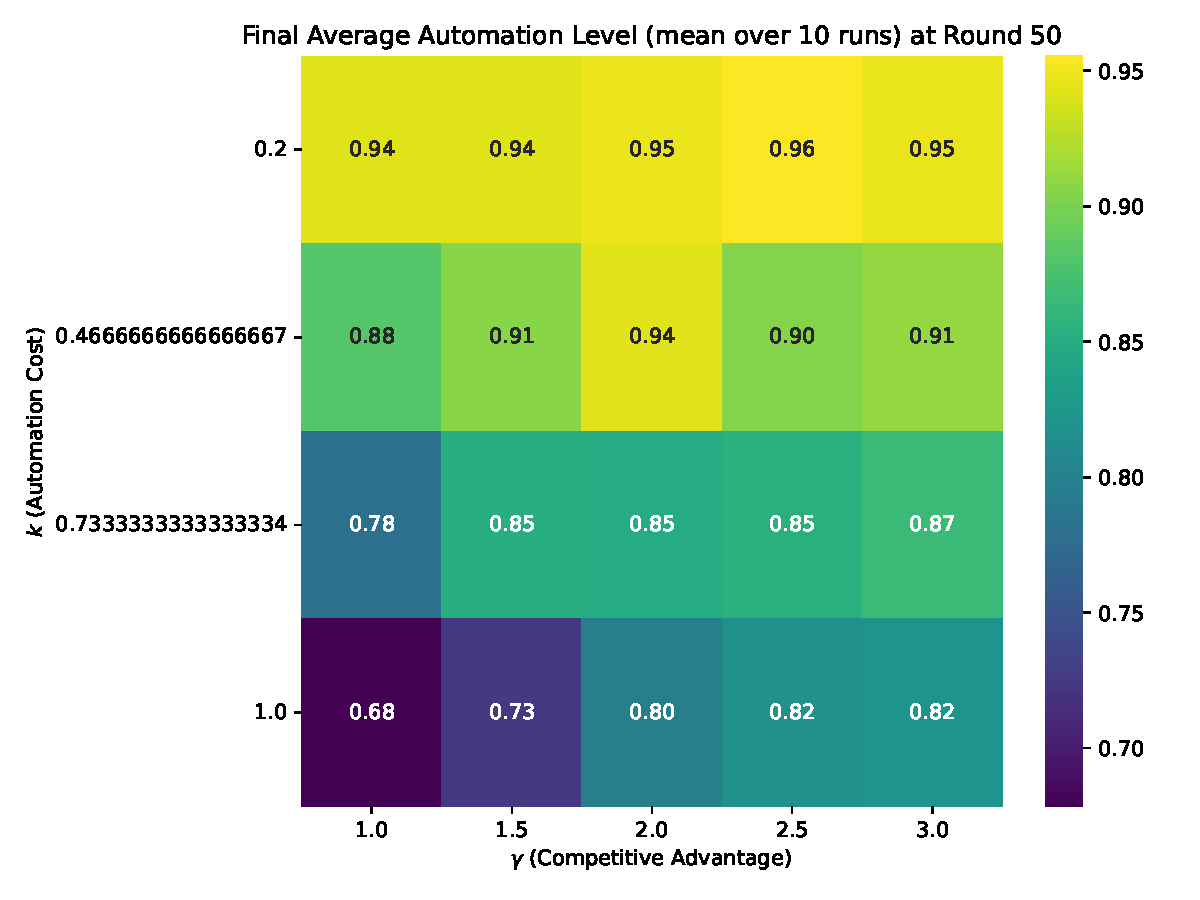
\includegraphics[width=0.8\textwidth]{final_automation_heatmap.pdf}
    \caption{Final Automation Heatmap}
    \label{fig:heatmap}
\end{figure}

\begin{figure}[h]
    \centering
    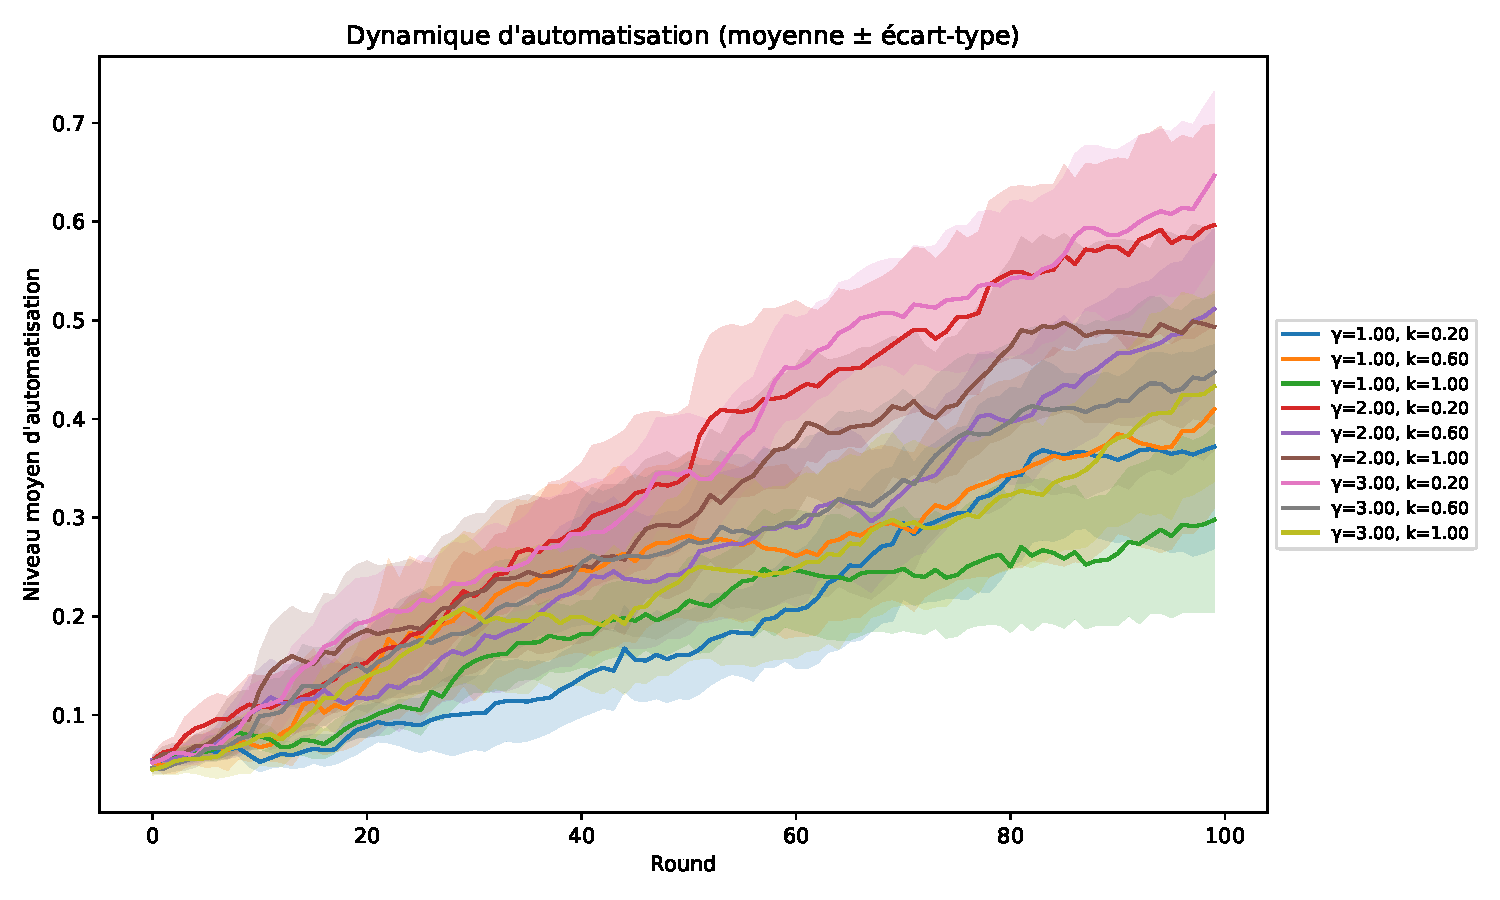
\includegraphics[width=0.8\textwidth]{automation_dynamics_stddev.pdf}
    \caption{Automation Dynamics with Standard Deviation}
    \label{fig:dynamics}
\end{figure}

\subsection{Macroeconomic Consequences}
Labor displacement drives unemployment \(u \to 0.6\) over the simulation duration. Without redistribution, aggregate consumption collapses by roughly 60\%, leading to contraction despite rising gross output. The fall in consumer demand destabilizes GDP growth, corroborating the paradox of abundance.

\subsection{Redistribution Effects on Demand and Social Indicators}
UBI stabilizes consumption by maintaining minimum income \(R\), reducing demand volatility but with neutral impact on social engagement. MBI similarly stabilizes demand, but simulations show a 20\% increase in simulated civic participation and education indices compared to UBI scenarios, suggesting positive social externalities.

\section{Discussion}

\subsection{The Paradox of Abundance and Market Failure}
Our results suggest structural market limitations under AGI: productivity growth becomes decoupled from demand as labor income collapses. Without redistribution, market equilibria may be unsustainable, foreshadowing potential crisis. Legacy labor-linked redistribution mechanisms may be inadequate due to shrinking tax bases and scalable exclusion \cite{MIT2025}.

\subsection{Merit-Based Income: Cultural and Institutional Dimensions}
MBI’s conditioning of income on certified knowledge may revitalize social recognition mechanisms beyond monetary rewards for labor. This could foster norms of lifelong learning, political participation, and social cohesion, potentially preparing society for post-economic realities where value stems from collective well-being and creativity. MBI may also offer political feasibility advantages over UBI in meritocratic cultures and align with psychological needs for contribution recognition.

\subsection{Policy Innovation and Ecological Sustainability}
Effective policy may need to integrate income stabilization with proactive education reform, ecological constraints, and expanded democratic participation (e.g., Citizens’ Initiatives). Circular economy principles could reconcile growth with finite resource limits. Together, these compose a multi-dimensional governance approach that may be essential for a just, sustainable transition.

\section{Conclusion}
Our integrated modeling of AGI-driven automation outlines potential systemic risks without income redistribution. Universal Basic Income and Merit-Based Income are presented as possible tools, with MBI uniquely positioning society for deeper cultural transformation toward a post-economic paradigm. Future research should refine simulation granularity, explore heterogeneous populations, and design implementable policies combining fiscal, social, and environmental dimensions.

\bibliographystyle{plain}
\bibliography{refs}

\end{document}
